\documentclass[11pt]{article}       % The percent symbol in your code starts a comment.  The comment ends at the next linebreak.
\usepackage[english]{babel}         % Packages add functionality and style conventions to your documents. Don't edit this section!
\usepackage{fullpage}               % Eliminates wasted space
\usepackage[utf8]{inputenc}         % Necessary for character encoding
\usepackage{amsmath, amssymb,amsthm}% Required math packages
\usepackage{graphicx}               % For handling graphics
\usepackage[colorinlistoftodos]{todonotes}  % For the fancy "todo" stuff
\usepackage{hyperref}               % For clickable links in the final PDF
\usepackage{tikz}
\theoremstyle{definition}
\newtheorem{theorem}{Theorem}
\newtheorem{lemma}[theorem]{Lemma}
\newtheorem{prop}[theorem]{Proposition}
\newtheorem{claim}[theorem]{Claim}

\title{Complex Analysis -- Homework \#7}

\author{ Komissar, Feldman, Kallus }

\date{ Due Friday, February 19 }

\begin{document}
\pagecolor{black}
\color{white}
\maketitle

\noindent{\bf 1. }  Let $f\left(x\right)=\dfrac{1}{1-x+3x^2}$.   Find the real polynomial $q\left(x\right) = q_0 + q_1x + q_2x^2 +q_3x^3$  that agrees with $f$ at the \emph{Chebyshev nodes} that you found as the roots of the polynomial $T_4$ in problem {\bf 3} of {\bf Homework \#6}; this is another \emph{cubic interpolant of $f$}, this time for the given Chebyshev nodes.  As before, indicate the set-up for your approach, but you need not include every step of the derivation, and certainly employ technology to perform computations.

\medskip
We need to solve this system of equations:
\begin{align*}
    f\left(\frac{\sqrt{2-\sqrt2}}2\right) &= q_0 + q_1\left(\frac{\sqrt{2-\sqrt2}}2\right) + q_2\left(\frac{\sqrt{2-\sqrt2}}2\right)^2 + q_3\left(\frac{\sqrt{2-\sqrt2}}2\right)^3 \\
    f\left(\frac{\sqrt{2+\sqrt2}}2\right) &= q_0 + q_1\left(\frac{\sqrt{2+\sqrt2}}2\right) + q_2\left(\frac{\sqrt{2+\sqrt2}}2\right)^2 + q_3\left(\frac{\sqrt{2+\sqrt2}}2\right)^3 \\
    f\left(-\frac{\sqrt{2-\sqrt2}}2\right) &= q_0 + q_1\left(-\frac{\sqrt{2-\sqrt2}}2\right) + q_2\left(-\frac{\sqrt{2-\sqrt2}}2\right)^2 + q_3\left(-\frac{\sqrt{2-\sqrt2}}2\right)^3 \\
    f\left(-\frac{\sqrt{2+\sqrt2}}2\right) &= q_0 + q_1\left(-\frac{\sqrt{2+\sqrt2}}2\right) + q_2\left(-\frac{\sqrt{2+\sqrt2}}2\right)^2 + q_3\left(-\frac{\sqrt{2+\sqrt2}}2\right)^3
\end{align*}

This is pretty easy with Wolfram$|$Alpha:
\begin{align*}
    q_0 &= \frac{1224}{1457}, \\
    q_1 &= \frac{888}{1457}, \\
    q_2 &=-\frac{920}{1457}, \\
    q_3 &=-\frac{896}{1457}.
\end{align*}

Thus, $$q(x) = \frac{1224}{1457} + \frac{888}{1457}x - \frac{920}{1457}x^2 - \frac{896}{1457}x^3.$$

\newpage
\vskip.1in
\hrule
\vskip.1in

\noindent{\bf 2. }  Referring to the polynomials $p$ from {\bf Homework \#7}  and $q$ from the present {\bf Homework \#8}:
\vskip.1in
\noindent {\bf a. }  On the same set of coordinate axes, provide computer-generated graphs of both $f$ and $q$ on the interval $[-1,1]$.

\begin{center}
($f$ is shown in red, and $q$ is shown in pink.)
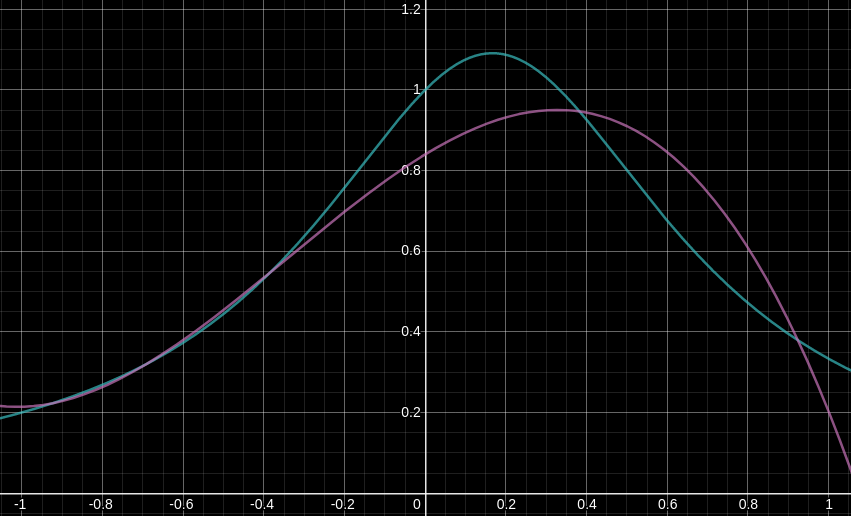
\includegraphics[scale=.5]{f-q.png}
\end{center}

\vskip.1in
\noindent {\bf b. }  On the same set of coordinate axes, provide computer-generated graphs of both $|f-p|$ and $|f-q|$ on the interval $[-1,1]$.  Note which of the two differences reaches a lower maximum.

\begin{center}
($|f-p|$ is shown in pink, and $|f-q|$ is shown in olive.)
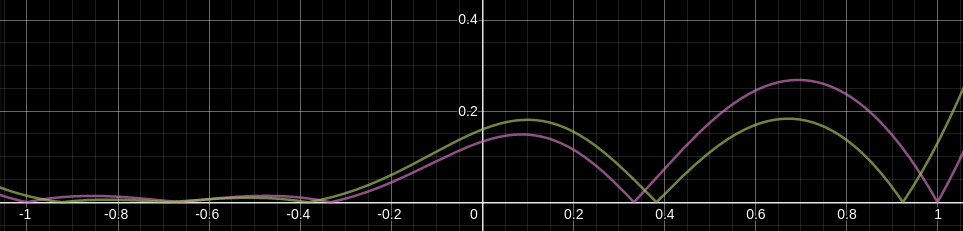
\includegraphics[scale=.5]{fp-fq.png}
\end{center}

$|f-q|$ has a lower maximum than $|f-p|$ on that interval $[-1,1]$.

\vskip.1in
\hrule

\end{document}